\section{Data} \label{Data}

\subsection{Ultra Short Tenor Options} \label{3_ultra_short_tenor}

\begin{figure}
    \centering
    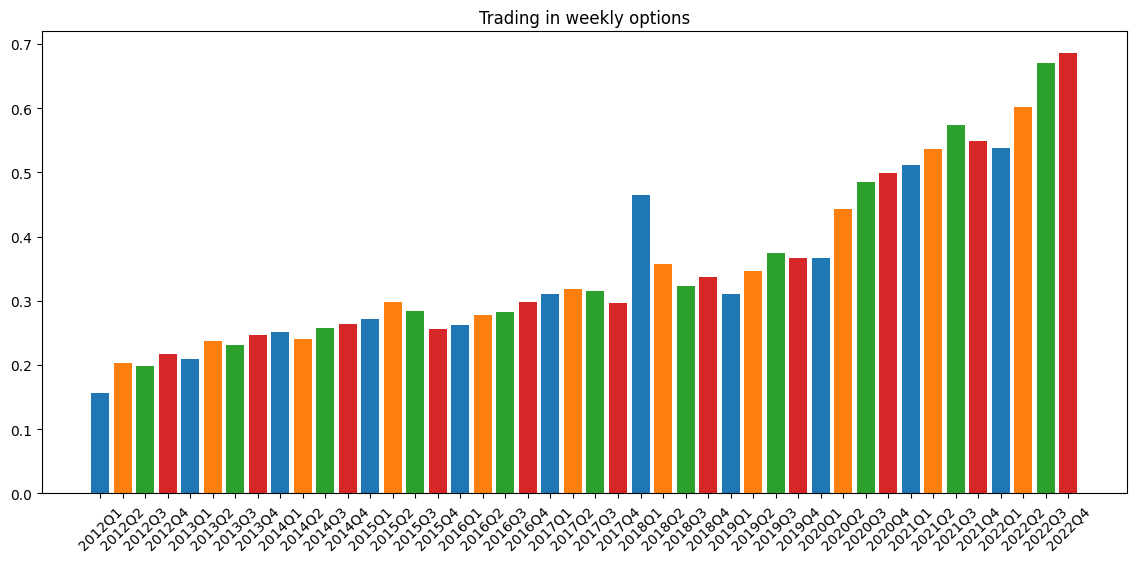
\includegraphics[width=\linewidth]{figures/option_volume.png}
    \caption{\textit{The number of contracts traded in Weekly SPX options (with a tenor less or equal to 5 trading days) per quarter as a fraction of total volume for options with a maturity up to one year. The data covers the period from 2012 to 2022. Data source: OptionMetrics}}
    \label{3_options_volume}
\end{figure}

Figure \ref{3_options_volume} shows the rising trend in the scale of weekly options trading. In the past few years, weekly options have made up the majority of total trading volume. There are several reasons that can explain this phenomenon: first, the past years were filled with economic downturns and periods of recovery and economic growth, which has led to increased demands for options, for both hedging and speculative purposes. Second, the federal reserve implemented policies of quantitative easing, allowing US citizens easy access to capital. This has led to a rise in the amount of retail investors, whom are also active in weekly options trading. Third, by 2022, the CBOE has expanded their zero-day-to-expiration (0DTE) options to every trading day of the week, which increased the volume traded in 0DTE options. 

For our study, we consider the time period 2020 till 2022. The period is rich in economic events: with the pandemic prompting global supply chain disruptions and lockdowns, to the implementation quantitative easing by central banks, and reports of rising inflation. 

[For firms specifically: oil prices, war, rise of AI, among others]

We obtain European options data using the database of OptionMetrics. For every trading day, we obtain the data of the ultra short tenor options by filtering for options with less or equal to 5 business days. We obtain the strike price, time to maturity, trading volume, best bid, and best ask price of the options. The mid price is then taken as a measure of the option price. We omit the options that are far in, or far out-of-the money, that show low trading volumes, as the price for those option are either the pay-off itself or close to 0, adding little information to the implied volatility. For the SPX options, we obtain a total of 823,118 observations. [Decide on a training, validation, and test set (initial idea: 70\% train, 10\% validation, 20\% test, while retaining the time-series structure)]

%First: options data
%time period, maturities, 

In addition to SPX options, we consider several individual stocks in Table \ref{3_macro_variables} to evaluate the effectiveness of our methods. We argue that the stocks chosen can be affected by news data, by both articles on the company itself, and sector-wide news. 
S\&P500 first, then individual stocks

\begin{table}[]
    \centering
    \begin{tabular}{ccc}
        \hline
        Company Name & Ticker & Sector  \\
        \hline
        Apple inc & AAPL & Technology \\
        NVIDIA & NVDA & Technology \\
        Shell PLC & SHELL & Energy \\
        Exxonmobil & XOM & Energy \\
        Boeing & BA & Industrial \\
        \hline
        
    \end{tabular}
    \caption{Different stocks along with their ticker and sector, selected for our IVS model}
    \label{3_stocks}
\end{table}

\subsection{Macro Economic Variables and Events} \label{3_macro_data}
\begin{table}[]
    \centering
    \begin{tabular}{cc}
         \hline 
         Macro variable & Source \\
         \hline
         Gross Domestic Product & FRED \\
         Unemployment rate & FRED \\
         Inflation rate & FRED \\
         Risk free Interest rate & FRED \\
         M1 money supply & FRED \\
         M2 money supply & FRED \\
         Nominal house prices & [...] \\
         ... & \\
         \hline
         
    \end{tabular}
    \caption{Overview of the quarterly macro-economic data considered in the study}
    \label{3_macro_variables}
\end{table}

News and text data - obtain amount of articles through the New York Times API (have to figure how to go smart about this, but searching using keywords will likely be the approach )

FinBERT - demonstrate the embeddings

\subsection{Idiosyncratic Variables and News} \label{3_stock_data}

In addition to the macro events, we consider firm-specific data for the estimation of the ultra short tenor option of the singular stocks. We obtain the daily stock price data using the CRSP database, and retrieve accounting variables by going through the quarterly report of each individual company. An overview of the accounting variables is given in Table \ref{3_accounting variables}

\begin{table}[]
    \centering
    \begin{tabular}{c}
         \hline 
         Variable \\
         \hline
         Total assets \\
         Current assets \\
         Cash flow \\
         Total liabilities \\
         Current liabilities \\
         Sales \\
         EBITDA \\
         \hline
          
    \end{tabular}
    \caption{Accounting variables considered for each stock}
    \label{3_accounting variables}
\end{table}

Singular stock news data; rumors and announcements can influence the volatility of the stock. Examples: Apple supply chain disruptions, advancements in AI improves NVIDIA earnings, Court cases against Shell regarding climate change, reports of Boeing aircrafts falling apart during flights, announcements of Exxonmobil stumbling upon new oil fields. Obtain the text data from financial news (The financial times, or The New York times, (check other literature, what they have done ))

[Provide overview of number of articles per stock, and their wordcount in a Table here]
